\documentclass[unicode,11pt,a4paper,oneside,numbers=endperiod,openany]{scrartcl}

\usepackage{assignment}
\usepackage{textcomp}
\usepackage{graphicx} 
\usepackage{rotating}
\usepackage{auto-pst-pdf}
\usepackage{float}

\begin{document}

\setassignment
\setduedate{15 October 2019, 13:30}

\serieheader{High Performance Computing}{2019}{Student: Gabriel Fernandes de Oliveira}{Discussed with: N/A}{Solution for Assignment 2}{}
\newline

In this exercise you will practice in data access optimization and performance-oriented programming for cluster environments.


\section{Explaning memory hierarchies \punkte{30}}

    \begin{enumerate}
        \item  The following data was found using the likwid module and the meminfo file, as suggested by the exercise.\\
            \begin{tabular}{| l || c |}
                \hline
                Main memory & 65.69 GB \\ 
                \hline
                L3 cache & 20 MB \\
                \hline
                L2 cache & 256 kB \\
                \hline 
                L1 cache & 32 kB \\
                \hline
            \end{tabular}
        \item  Both graphs were created and added to this assignment: 

        \begin{figure}[H]
            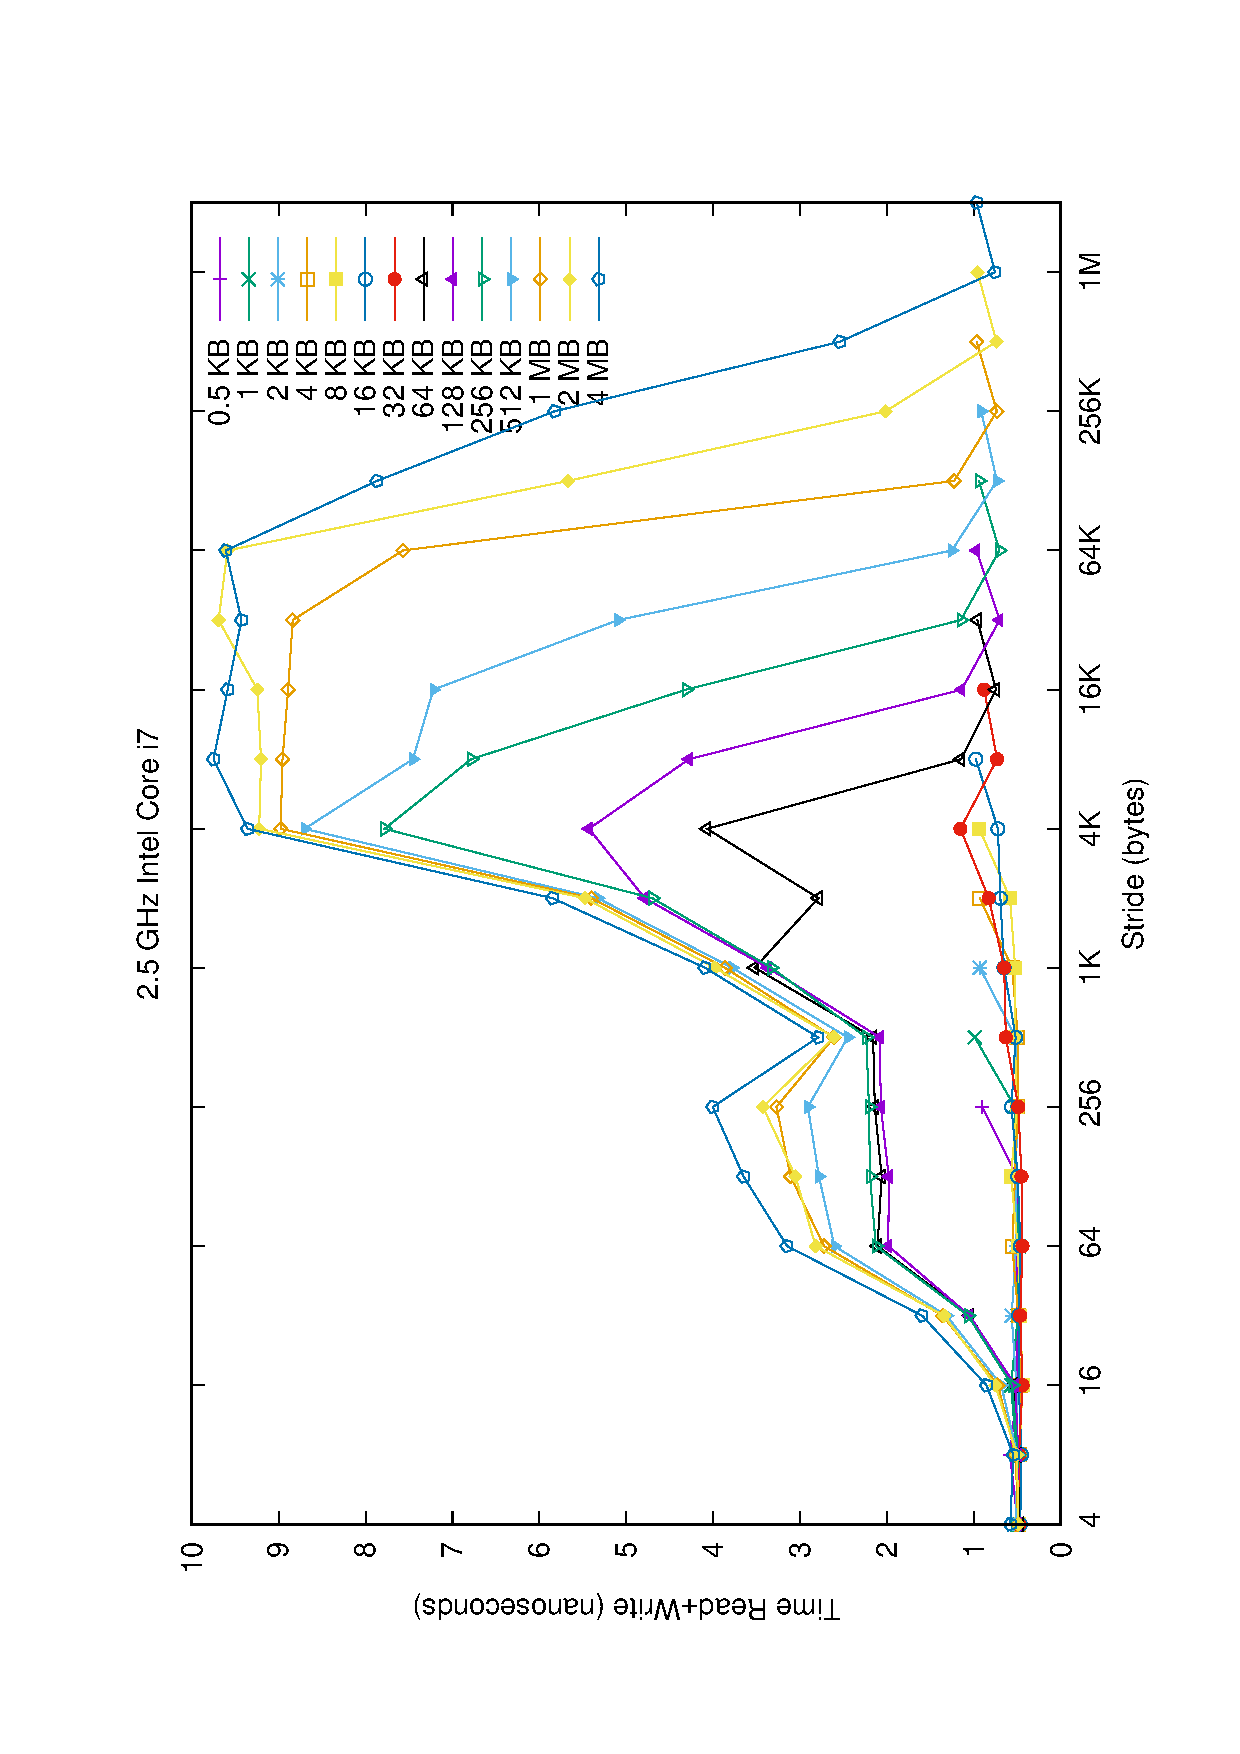
\includegraphics[width=\linewidth]{./membench/generic_mac.pdf}
            \caption{This is the graph generated for my Macbook Pro running on macOS Sierra 10.12.6}
        \end{figure}
        \begin{figure}[H]
            \includegraphics[width=\linewidth]{./membench/generic_icsmaster.pdf}
            \caption{Graph generated on icsmaster}
        \end{figure}
           
        The ps files were also added to this assignment folder, they are called respectivelly generic\_mac.ps and generic\_icsmaster.ps.

        \item 
            \begin{itemize}
                \item $csize = 128 = 0.5kB$ and $stride = 1 = 4B$
                    This example has a very good performance, around 0.5ns for both icsmaster and my computer, that is mainly due to the good spatial locality associated with a small value of stride.
                    Because the stride is $1$, every element loaded in a cache line will be used, hence the good spatial locality and performance of this case.

                \item $csize = 2^{20} = 4MB$ and $stride = csize/2 = 2^{19} = 2MB$
                    This is another extreme case with a good performance, the read+write takes about 1ns for both computers, that is due to the temporal locality associated with traversing the same elements already loaded on cache.
                    
                    Since the stride is half the size of the array only two elements of the array are being accessed every time the array is traversed.
                    On the first array traversal these two elements are loaded into the cache, and on all following traversals they are retrieved directly from cache, hence the good temporal locality and performance also visible in this case.
            \end{itemize}

        \item  The points with best temporal locality in the graph are the ones closes to the end of each line.
            For example, for the array of size $4MB$, the stride values $2MB$ and $1MB$ offer a very good temporal locality.
            This happens because with a large stride value, few elements of the array are accessed. 
            These few elements accessed can all fit into the cache, and are reused many times since the array is being traversed multiple times, hence the good temporal locality and the high performance on these conditions.

            One can notice similar high performances on other array sizes, when the stride value is close to half or a quarter of the array size.

            Another example of good temporal locality happens for small array sizes ($\leq 32KB$), since these arrays can be fully stored on the L1 cache.
            The first time that the array is traversed every element is loaded into the cache, then for every following traversal the whole array is on cache, so the cache elements are simply reused.

    \end{enumerate}

    \section{Optimize Square Matrix-Matrix Multiplication  \punkte{70}}

\end{document}
